\documentclass{beamer}

\usepackage[T1]{fontenc}   % required for luximono!
\usepackage{lmodern}
\usepackage[scaled=0.8]{luximono}  % typewriter font with bold face

% To install the luximono font files:
% getnonfreefonts-sys --all        or
% getnonfreefonts-sys luximono
%
% when there are trouble you might need to:
% - Create /etc/texmf/updmap.d/99local-luximono.cfg
%   containing the single line: Map ul9.map
% - Run update-updmap followed by mktexlsr and updmap-sys
%
% This commands must be executed as root with a root environment
% (i.e. run "sudo su" and then execute the commands in the root
% shell, don't just prefix the commands with "sudo").

% formats the text accourding the set language
\usepackage[english]{babel}
\usepackage{amsmath}
\usepackage{multirow}
\usepackage{booktabs}
\usepackage{listings}
\usepackage{skull}

\usepackage{tikz}
\usetikzlibrary{calc}
\usetikzlibrary{arrows}
\usetikzlibrary{scopes}
\usetikzlibrary{through}
\usetikzlibrary{shapes.geometric}

\lstset{basicstyle=\ttfamily}

\def\B#1{{\tt\textbackslash{}#1}}
\def\C#1{\lstinline[language=C++]{#1}}
\def\V#1{\lstinline[language=Verilog]{#1}}

\lstdefinelanguage{liberty}{
	morecomment=[s]{/*}{*/},
	morekeywords={library,cell,area,pin,direction,function,clocked_on,next_state,clock,ff},
	morestring=[b]",
}

\lstdefinelanguage{rtlil}{
	morecomment=[l]{\#},
	morekeywords={module,attribute,parameter,wire,memory,auto,width,offset,size,input,output,inout,cell,connect,switch,case,assign,sync,low,high,posedge,negedge,edge,always,update,process,end},
	morestring=[b]",
}

\title{Yosys Open SYnthesis Suite}
\author{Clifford Wolf}
\institute{http://www.clifford.at/}

\usetheme{Madrid}
\usecolortheme{seagull}
\beamertemplatenavigationsymbolsempty

\definecolor{YosysGreen}{RGB}{85,136,102}
\setbeamercolor{title}{fg=black,bg=YosysGreen!70}
\setbeamercolor{titlelike}{fg=black,bg=YosysGreen!70}
\setbeamercolor{frametitle}{fg=black,bg=YosysGreen!70}
\setbeamercolor{block title}{fg=black,bg=YosysGreen!70}
\setbeamercolor{item projected}{fg=black,bg=YosysGreen}

\begin{document}

\begin{frame}
\titlepage
\end{frame}

\setcounter{section}{-1}
\section{Outline}

\begin{frame}{Outline}
Yosys is an Open Source Verilog synthesis tool, and more.

\bigskip
Outline of this presentation:
\begin{itemize}
\item Introduction to the field and Yosys
\item Yosys usage examples (synthesis)
\item Yosys usage examples (advanced synthesis)
\item Yosys usage examples (beyond synthesis)
\item Programming Yosys extensions
\end{itemize}
\end{frame}


\section{Introduction}

\begin{frame}
\sectionpage
\end{frame}

%%%%%%%%%%%%%%%%%%%%%%%%%%%%%%%%%%%%%%%%%%%%%%%%%%%%%%%%%%%%%%%%%%%%%%%%%%%%%

\subsection{Representations of (digital) Circuits}

\begin{frame}[t]{\subsecname}
\begin{itemize}
	\item Graphical
		\begin{itemize}
			\item \alert<1>{Schematic Diagram}
			\item \alert<2>{Physical Layout}
		\end{itemize}
	\bigskip
	\item Non-graphical
		\begin{itemize}
			\item \alert<3>{Netlists}
			\item \alert<4>{Hardware Description Languages (HDLs)}
		\end{itemize}
\end{itemize}
\bigskip
\begin{block}{Definition:
\only<1>{Schematic Diagram}%
\only<2>{Physical Layout}%
\only<3>{Netlists}%
\only<4>{Hardware Description Languages (HDLs)}}
\only<1>{
	Graphical representation of the circtuit topology. Circuit elements
	are represented by symbols and electrical connections by lines. The gometric
	layout is for readability only.
}%
\only<2>{
	The actual physical geometry of the device (PCB or ASIC manufracturing masks).
	This is the final product of the design process.
}%
\only<3>{
	A list of circuit elements and a list of connections. This is the raw circuit
	topology.
}%
\only<4>{
	Computer languages (like programming languages) that can be used to describe
	circuits. HDLs are much more powerful in describing huge circuits than
	schematic diagrams.
}%
\end{block}
\end{frame}

%%%%%%%%%%%%%%%%%%%%%%%%%%%%%%%%%%%%%%%%%%%%%%%%%%%%%%%%%%%%%%%%%%%%%%%%%%%%%

\subsection{Levels of Abstraction for Digital Circuits}

\begin{frame}[t]{\subsecname}
\begin{itemize}
	\item \alert<1>{System Level}
	\item \alert<2>{High Level}
	\item \alert<3>{Behavioral Level}
	\item \alert<4>{Register-Transfer Level (RTL)}
	\item \alert<5>{Logical Gate Level}
	\item \alert<6>{Physical Gate Level}
	\item \alert<7>{Switch Level}
\end{itemize}
\bigskip
\begin{block}{Definition:
\only<1>{System Level}%
\only<2>{High Level}%
\only<3>{Behavioral Level}%
\only<4>{Register-Transfer Level (RTL)}%
\only<5>{Logical Gate Level}%
\only<6>{Physical Gate Level}%
\only<7>{Switch Level}}
\only<1>{
	Overall view of the circuit: E.g. block-diagrams or instruction-set architecture descriptions
}%
\only<2>{
	Functional implementation of circuit in high-level programming language (C, C++, SystemC, Matlab, Python, etc.).
}%
\only<3>{
	Cycle-accurate description of circuit in hardware description language (Verilog, VHDL, etc.).
}%
\only<4>{
	List of registers (flip-flops) and logic functions that calculate the next state from the previous one. Usually
	a netlist utilizing high-level cells such as adders, multiplieres, multiplexer, etc.
}%
\only<5>{
	Netlist of single-bit registers and basic logic gates (such as AND, OR,
	NOT, etc.). Popular form: And-Inverter-Graphs (AIGs) with pairs of primary
	inputs and outputs for each register bit.
}%
\only<6>{
	Netlist of cells that actually are available on the target architecture
	(such as CMOS gates in an ASCI or LUTs in an FPGA). Optimized for
	area and/or and/or speed (static timing or number of logic levels).
}%
\only<7>{
	Netlist of individual transistors.
}%
\end{block}
\end{frame}

%%%%%%%%%%%%%%%%%%%%%%%%%%%%%%%%%%%%%%%%%%%%%%%%%%%%%%%%%%%%%%%%%%%%%%%%%%%%%

\subsection{Digital Circuit Synthesis}

\begin{frame}{\subsecname}
	Synthesis Tools (such as Yosys) can transform HDL code to circuits:

	\bigskip
	\begin{center}
	\begin{tikzpicture}[scale=0.8, every node/.style={transform shape}]
			\tikzstyle{lvl} = [draw, fill=MyBlue, rectangle, minimum height=2em, minimum width=15em]
			\node[lvl] (sys) {System Level};
			\node[lvl] (hl) [below of=sys] {High Level};
			\node[lvl] (beh) [below of=hl] {Behavioral Level};
			\node[lvl] (rtl) [below of=beh] {Register-Transfer Level (RTL)};
			\node[lvl] (lg) [below of=rtl] {Logical Gate Level};
			\node[lvl] (pg) [below of=lg] {Physical Gate Level};
			\node[lvl] (sw) [below of=pg] {Switch Level};

			\draw[dotted] (sys.east)  -- ++(1,0) coordinate (sysx);
			\draw[dotted] (hl.east)  -- ++(1,0) coordinate (hlx);
			\draw[dotted] (beh.east) -- ++(1,0) coordinate (behx);
			\draw[dotted] (rtl.east) -- ++(1,0) coordinate (rtlx);
			\draw[dotted] (lg.east)  -- ++(1,0) coordinate (lgx);
			\draw[dotted] (pg.east)  -- ++(1,0) coordinate (pgx);
			\draw[dotted] (sw.east)  -- ++(1,0) coordinate (swx);

			\draw[gray,|->] (sysx) -- node[right] {System Design} (hlx);
			\draw[|->|] (hlx) -- node[right] {High Level Synthesis (HLS)} (behx);
			\draw[->|] (behx) -- node[right] {Behavioral Synthesis} (rtlx);
			\draw[->|] (rtlx) -- node[right] {RTL Synthesis} (lgx);
			\draw[->|] (lgx) -- node[right] {Logic Synthesis} (pgx);
			\draw[gray,->|] (pgx) -- node[right] {Cell Library} (swx);

			\draw[dotted] (behx) -- ++(4,0) coordinate (a);
			\draw[dotted] (pgx) -- ++(4,0) coordinate (b);
			\draw[|->|] (a) -- node[right] {Yosys} (b);
	\end{tikzpicture}
	\end{center}
\end{frame}

%%%%%%%%%%%%%%%%%%%%%%%%%%%%%%%%%%%%%%%%%%%%%%%%%%%%%%%%%%%%%%%%%%%%%%%%%%%%%

\subsection{What Yosys can and can't do}

\begin{frame}{\subsecname}

Things Yosys can do:
\begin{itemize}
\item Read and process (most of) modern Verilog-2005 code.
\item Perform all kinds of operations on netlist (RTL, Logic, Gate).
\item Perform logic optimiziations and gate mapping with ABC\footnote[frame]{\url{http://www.eecs.berkeley.edu/~alanmi/abc/}}.
\end{itemize}

\bigskip
Things Yosys can't do:
\begin{itemize}
\item Process high-level languages such as C/C++/SystemC.
\item Create physical layouts (place\&route).
\end{itemize}

\bigskip
A typical flow combines Yosys with with a low-level implementation tool, such
as Qflow\footnote[frame]{\url{http://opencircuitdesign.com/qflow/}} for ASIC designs.

\end{frame}

%%%%%%%%%%%%%%%%%%%%%%%%%%%%%%%%%%%%%%%%%%%%%%%%%%%%%%%%%%%%%%%%%%%%%%%%%%%%%

\subsection{Yosys Data- and Control-Flow}

\begin{frame}{\subsecname}
	A (usually short) synthesis script controlls Yosys.

	This scripts contain three types of commands:
	\begin{itemize}
	\item {\bf Frontends}, that read input files (usually Verilog).
	\item {\bf Passes}, that perform transformation on the design in memory.
	\item {\bf Backends}, that write the design in memory to a file (various formats are available, e.g. Verilog, BLIF, EDIF, SPICE, BTOR, etc.).
	\end{itemize}

	\bigskip
	\begin{center}
	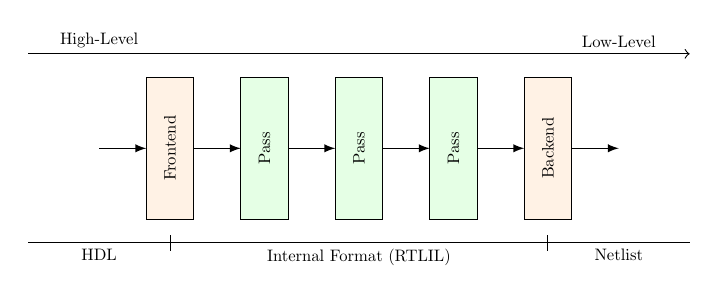
\begin{tikzpicture}[scale=0.6, every node/.style={transform shape}]
		\path (-1.5,3) coordinate (cursor);
		\draw[-latex] ($ (cursor) + (0,-1.5) $) -- ++(1,0);
		\draw[fill=orange!10] ($ (cursor) + (1,-3) $) rectangle node[rotate=90] {Frontend} ++(1,3) coordinate (cursor);
		\draw[-latex] ($ (cursor) + (0,-1.5) $) -- ++(1,0);
		\draw[fill=green!10] ($ (cursor) + (1,-3) $) rectangle node[rotate=90] {Pass} ++(1,3) coordinate (cursor);
		\draw[-latex] ($ (cursor) + (0,-1.5) $) -- ++(1,0);
		\draw[fill=green!10] ($ (cursor) + (1,-3) $) rectangle node[rotate=90] {Pass} ++(1,3) coordinate (cursor);
		\draw[-latex] ($ (cursor) + (0,-1.5) $) -- ++(1,0);
		\draw[fill=green!10] ($ (cursor) + (1,-3) $) rectangle node[rotate=90] {Pass} ++(1,3) coordinate (cursor);
		\draw[-latex] ($ (cursor) + (0,-1.5) $) -- ++(1,0);
		\draw[fill=orange!10] ($ (cursor) + (1,-3) $) rectangle node[rotate=90] {Backend} ++(1,3) coordinate (cursor);
		\draw[-latex] ($ (cursor) + (0,-1.5) $) -- ++(1,0);

		\path (-3,-0.5) coordinate (cursor);
		\draw (cursor) -- node[below] {HDL} ++(3,0) coordinate (cursor);
		\draw[|-|] (cursor) -- node[below] {Internal Format (RTLIL)} ++(8,0) coordinate (cursor);
		\draw (cursor) -- node[below] {Netlist} ++(3,0);

		\path (-3,3.5) coordinate (cursor);
		\draw[-] (cursor) -- node[above] {High-Level} ++(3,0) coordinate (cursor);
		\draw[-] (cursor) -- ++(8,0) coordinate (cursor);
		\draw[->] (cursor) -- node[above] {Low-Level} ++(3,0);
	\end{tikzpicture}
	\end{center}
\end{frame}

%%%%%%%%%%%%%%%%%%%%%%%%%%%%%%%%%%%%%%%%%%%%%%%%%%%%%%%%%%%%%%%%%%%%%%%%%%%%%

\subsection{Program Components and Data Formats}

\begin{frame}{\subsecname}
	\begin{center}
	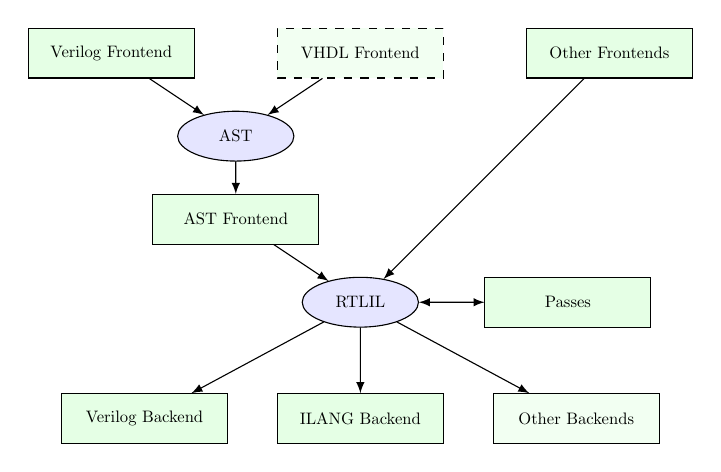
\begin{tikzpicture}[scale=0.6, every node/.style={transform shape}]
		\tikzstyle{process} = [draw, fill=green!10, rectangle, minimum height=3em, minimum width=10em, node distance=15em]
		\tikzstyle{data} = [draw, fill=blue!10, ellipse, minimum height=3em, minimum width=7em, node distance=15em]
		\node[process] (vlog) {Verilog Frontend};
		\node[process, dashed, fill=green!5] (vhdl) [right of=vlog] {VHDL Frontend};
		\node[process] (ilang) [right of=vhdl] {Other Frontends};
		\node[data] (ast) [below of=vlog, node distance=5em, xshift=7.5em] {AST};
		\node[process] (astfe) [below of=ast, node distance=5em] {AST Frontend};
		\node[data] (rtlil) [below of=astfe, node distance=5em, xshift=7.5em] {RTLIL};
		\node[process] (pass) [right of=rtlil, node distance=5em, xshift=7.5em] {Passes};
		\node[process] (vlbe) [below of=rtlil, node distance=7em, xshift=-13em] {Verilog Backend};
		\node[process] (ilangbe) [below of=rtlil, node distance=7em, xshift=0em] {ILANG Backend};
		\node[process, fill=green!5] (otherbe) [below of=rtlil, node distance=7em, xshift=+13em] {Other Backends};

		\draw[-latex] (vlog) -- (ast);
		\draw[-latex] (vhdl) -- (ast);
		\draw[-latex] (ast) -- (astfe);
		\draw[-latex] (astfe) -- (rtlil);
		\draw[-latex] (ilang) -- (rtlil);
		\draw[latex-latex] (rtlil) -- (pass);
		\draw[-latex] (rtlil) -- (vlbe);
		\draw[-latex] (rtlil) -- (ilangbe);
		\draw[-latex] (rtlil) -- (otherbe);
	\end{tikzpicture}
	\end{center}
\end{frame}

%%%%%%%%%%%%%%%%%%%%%%%%%%%%%%%%%%%%%%%%%%%%%%%%%%%%%%%%%%%%%%%%%%%%%%%%%%%%%

\subsection{Example Problem}

\begin{frame}[fragile]{\subsecname{} -- Verilog Source: \tt counter.v}
\lstinputlisting[xleftmargin=1cm, language=Verilog]{PRESENTATION_Intro/counter.v}
\end{frame}

\begin{frame}[fragile]{\subsecname{} -- Cell Library: \tt mycells.lib}
\begin{columns}
\column[t]{5cm}
\lstinputlisting[basicstyle=\ttfamily\fontsize{8pt}{10pt}\selectfont, language=liberty, lastline=20]{PRESENTATION_Intro/mycells.lib}
\column[t]{5cm}
\lstinputlisting[basicstyle=\ttfamily\fontsize{8pt}{10pt}\selectfont, language=liberty, firstline=21]{PRESENTATION_Intro/mycells.lib}
\end{columns}
\end{frame}

%%%%%%%%%%%%%%%%%%%%%%%%%%%%%%%%%%%%%%%%%%%%%%%%%%%%%%%%%%%%%%%%%%%%%%%%%%%%%

\subsection{Example Synthesis Script}

\begin{frame}[t]{\subsecname}

\setbeamercolor{alerted text}{fg=white,bg=red}

\begin{minipage}[t]{6cm}
\tt\scriptsize
\# read design\\
\boxalert<1>{read\_verilog counter.v}\\
\boxalert<2>{hierarchy -check -top counter}

\medskip
\# the high-level stuff\\
\boxalert<3>{proc}; \boxalert<4>{opt}; \boxalert<5>{memory}; \boxalert<6>{opt}; \boxalert<7>{fsm}; \boxalert<8>{opt}

\medskip
\# mapping to internal cell library\\
\boxalert<9>{techmap}; \boxalert<10>{opt}

\bigskip
\it continued\dots
\end{minipage}
\begin{minipage}[t]{5cm}
\tt\scriptsize
\# mapping flip-flops to mycells.lib\\
\boxalert<11>{dfflibmap -liberty mycells.lib}

\medskip
\# mapping logic to mycells.lib\\
\boxalert<12>{abc -liberty mycells.lib}

\medskip
\# cleanup\\
\boxalert<13>{clean}

\medskip
\# write synthesized design\\
\boxalert<14>{write\_verilog synth.v}
\end{minipage}

\vskip1cm

\begin{block}{Command: \tt
\only<1>{read\_verilog counter.v}%
\only<2>{hierarchy -check -top counter}%
\only<3>{proc}%
\only<4>{opt}%
\only<5>{memory}%
\only<6>{opt}%
\only<7>{fsm}%
\only<8>{opt}%
\only<9>{techmap}%
\only<10>{opt}%
\only<11>{dfflibmap -liberty mycells.lib}%
\only<12>{abc -liberty mycells.lib}%
\only<13>{clean}%
\only<14>{write\_verilog synth.v}}
\only<1>{
	Read Verilog source file and convert to internal representation.
}%
\only<2>{
	Elaborate the design hierarchy. Should alsways be the first
	command after reading the design.
}%
\only<3>{
	Convert ``processes'' (the internal representation of behavioral
	Verilog code) into multiplexers and registers.
}%
\only<4>{
	Perform some basic optimizations and cleanups.
}%
\only<5>{
	Analyze memories and create circuits to implement them.
}%
\only<6>{
	Perform some basic optimizations and cleanups.
}%
\only<7>{
	Analyze and optimize finite state machines.
}%
\only<8>{
	Perform some basic optimizations and cleanups.
}%
\only<9>{
	Map coarse-grain RTL cells (adders, etc.) to fine-grain
	logic gates (AND, OR, NOT, etc.).
}%
\only<10>{
	Perform some basic optimizations and cleanups.
}%
\only<11>{
	Map registers to available hardware flip-flops.
}%
\only<12>{
	Map logix to available hardware gates.
}%
\only<13>{
	Clean up the design (just the last step of {\tt opt}).
}%
\only<14>{
	Write final synthesis result to output file.
}%
\end{block}

\end{frame}

%%%%%%%%%%%%%%%%%%%%%%%%%%%%%%%%%%%%%%%%%%%%%%%%%%%%%%%%%%%%%%%%%%%%%%%%%%%%%

\subsection{Running the Synthesis Script}

\begin{frame}[t, fragile]{\subsecname{} -- Step 1/4}
\begin{verbatim}
read_verilog counter.v
hierarchy -check -top counter
\end{verbatim}

\vfill
\includegraphics[width=\linewidth,trim=0 0cm 0 0cm]{PRESENTATION_Intro/counter_00.pdf}
\end{frame}

\begin{frame}[t, fragile]{\subsecname{} -- Step 2/4}
\begin{verbatim}
proc; opt; memory; opt; fsm; opt
\end{verbatim}

\vfill
\includegraphics[width=\linewidth,trim=0 0cm 0 0cm]{PRESENTATION_Intro/counter_01.pdf}
\end{frame}

\begin{frame}[t, fragile]{\subsecname{} -- Step 3/4}
\begin{verbatim}
techmap; opt
\end{verbatim}

\vfill
\includegraphics[width=\linewidth,trim=0 0cm 0 0cm]{PRESENTATION_Intro/counter_02.pdf}
\end{frame}

\begin{frame}[t, fragile]{\subsecname{} -- Step 4/4}
\begin{verbatim}
dfflibmap -liberty mycells.lib
abc -liberty mycells.lib
clean
\end{verbatim}

\vfill
\includegraphics[width=\linewidth,trim=0 0cm 0 0cm]{PRESENTATION_Intro/counter_03.pdf}
\end{frame}

%%%%%%%%%%%%%%%%%%%%%%%%%%%%%%%%%%%%%%%%%%%%%%%%%%%%%%%%%%%%%%%%%%%%%%%%%%%%%

\subsection{Yosys Commands}

\begin{frame}[fragile]{\subsecname{} 1/3 \hspace{0pt plus 1 filll} (excerpt)}
Command reference:
\begin{itemize}
\item Use ``{\tt help}'' for a command list and ``{\tt help \it command}'' for details.
\item Or run ``{\tt yosys -H}'' and ``{\tt yosys -h \it command}''.
\item Or go to \url{http://www.clifford.at/yosys/documentation.html}.
\end{itemize}

\bigskip
Commands for design navigation and investigation:
\begin{lstlisting}[xleftmargin=1cm, basicstyle=\ttfamily\fontsize{8pt}{10pt}\selectfont]
    cd                   a shortcut for 'select -module <name>'
    ls                   list modules or objects in modules
    dump                 print parts of the design in ilang format
    show                 generate schematics using graphviz
    select               modify and view the list of selected objects
\end{lstlisting}

\bigskip
Commands for executing scripts or entering interactive mode:
\begin{lstlisting}[xleftmargin=1cm, basicstyle=\ttfamily\fontsize{8pt}{10pt}\selectfont]
    shell                enter interactive command mode
    history              show last interactive commands
    script               execute commands from script file
    tcl                  execute a TCL script file
\end{lstlisting}
\end{frame}

\begin{frame}[fragile]{\subsecname{} 2/3 \hspace{0pt plus 1 filll} (excerpt)}
Commands for reading and elaborating the design:
\begin{lstlisting}[xleftmargin=1cm, basicstyle=\ttfamily\fontsize{8pt}{10pt}\selectfont]
    read_ilang           read modules from ilang file
    read_verilog         read modules from verilog file
    hierarchy            check, expand and clean up design hierarchy
\end{lstlisting}

\bigskip
Commands for high-level synthesis:
\begin{lstlisting}[xleftmargin=1cm, basicstyle=\ttfamily\fontsize{8pt}{10pt}\selectfont]
    proc                 translate processes to netlists
    fsm                  extract and optimize finite state machines
    memory               translate memories to basic cells
    opt                  perform simple optimizations
\end{lstlisting}

\bigskip
Commands for technology mapping:
\begin{lstlisting}[xleftmargin=1cm, basicstyle=\ttfamily\fontsize{8pt}{10pt}\selectfont]
    techmap              simple technology mapper
    abc                  use ABC for technology mapping
    dfflibmap            technology mapping of flip-flops
    hilomap              technology mapping of constant hi- and/or lo-drivers
    iopadmap             technology mapping of i/o pads (or buffers)
    flatten              flatten design
\end{lstlisting}
\end{frame}

\begin{frame}[fragile]{\subsecname{} 3/3 \hspace{0pt plus 1 filll} (excerpt)}
Commands for writing the results:
\begin{lstlisting}[xleftmargin=1cm, basicstyle=\ttfamily\fontsize{8pt}{10pt}\selectfont]
    write_blif           write design to BLIF file
    write_btor           write design to BTOR file
    write_edif           write design to EDIF netlist file
    write_ilang          write design to ilang file
    write_spice          write design to SPICE netlist file
    write_verilog        write design to verilog file
\end{lstlisting}

\bigskip
Script-Commands for standard synthesis tasks:
\begin{lstlisting}[xleftmargin=1cm, basicstyle=\ttfamily\fontsize{8pt}{10pt}\selectfont]
    synth_xilinx         synthesis for Xilinx FPGAs
\end{lstlisting}

\bigskip
... and many many more.
\end{frame}

%%%%%%%%%%%%%%%%%%%%%%%%%%%%%%%%%%%%%%%%%%%%%%%%%%%%%%%%%%%%%%%%%%%%%%%%%%%%%

\subsection{More Verilog Examples}

\begin{frame}[fragile]{\subsecname{} 1/3}
\begin{lstlisting}[xleftmargin=1cm, basicstyle=\ttfamily\fontsize{8pt}{10pt}\selectfont, language=Verilog]
module detectprime(a, y);
    input [4:0] a;
    output y;

    integer i, j;
    reg [31:0] lut;

    initial begin
        for (i = 0; i < 32; i = i+1) begin
            lut[i] = i > 1;
            for (j = 2; j*j <= i; j = j+1)
                if (i % j == 0)
                    lut[i] = 0;
        end
    end

    assign y = lut[a];
endmodule
\end{lstlisting}
\end{frame}

\begin{frame}[fragile]{\subsecname{} 2/3}
\begin{lstlisting}[xleftmargin=1cm, basicstyle=\ttfamily\fontsize{8pt}{10pt}\selectfont, language=Verilog]
module carryadd(a, b, y);
    parameter WIDTH = 8;
    input [WIDTH-1:0] a, b;
    output [WIDTH-1:0] y;

    genvar i;
    generate
        for (i = 0; i < WIDTH; i = i+1) begin:STAGE
            wire IN1 = a[i], IN2 = b[i];
            wire C, Y;
            if (i == 0)
                assign C = IN1 & IN2, Y = IN1 ^ IN2;
            else
                assign C = (IN1 & IN2) | ((IN1 | IN2) & STAGE[i-1].C),
                       Y = IN1 ^ IN2 ^ STAGE[i-1].C;
            assign y[i] = Y;
        end
    endgenerate
endmodule
\end{lstlisting}
\end{frame}

\begin{frame}[fragile]{\subsecname{} 3/3}
\begin{lstlisting}[xleftmargin=1cm, basicstyle=\ttfamily\fontsize{7pt}{8.5pt}\selectfont, language=Verilog]
module cam(clk, wr_enable, wr_addr, wr_data, rd_data, rd_addr, rd_match);
    parameter WIDTH = 8;
    parameter DEPTH = 16;
    localparam ADDR_BITS = $clog2(DEPTH);

    input clk, wr_enable;
    input [ADDR_BITS-1:0] wr_addr;
    input [WIDTH-1:0] wr_data, rd_data;
    output reg [ADDR_BITS-1:0] rd_addr;
    output reg rd_match;

    integer i;
    reg [WIDTH-1:0] mem [0:DEPTH-1];

    always @(posedge clk) begin
        rd_addr <= 'bx;
        rd_match <= 0;
        for (i = 0; i < DEPTH; i = i+1)
            if (mem[i] == rd_data) begin
                rd_addr <= i;
                rd_match <= 1;
            end
        if (wr_enable)
            mem[wr_addr] <= wr_data;
    end
endmodule
\end{lstlisting}
\end{frame}

\subsection{Verification}

\begin{frame}{\subsecname}
Contiously checking the correctness of Yosys and making sure that new features
do not break old ones is a high priority in Yosys.

\bigskip
There are two external test suites build for Yosys: VlogHammer and yosys-bigsim
(see next slides)

\bigskip
In addition to that, yosys comes with $\approx\!200$ test cases used in ``{\tt make test}''.

\bigskip
A debug build of Yosys also contains a lot of asserts and checks the integrity of
the internal state after each command.
\end{frame}

\begin{frame}[fragile]{\subsecname{} -- VlogHammer}
VlogHammer is a Verilog regression test suite developed to test the different
subsystems in Yosys by comparing them to each other and the implementations
generated by some proprietary tools (Xilinx Vivado, Xilinx XST, Altera Quartus II, ...).

\bigskip
Yosys Subsystems tested: Verilog frontend, const folding, const eval, technology mapping,
simulation models, SAT models.

\bigskip
Thousands of auto-generated test cases containing code such as:
\begin{lstlisting}[xleftmargin=1cm, basicstyle=\ttfamily\fontsize{8pt}{10pt}\selectfont, language=Verilog]
assign y9 = $signed(((+$signed((^(6'd2 ** a2))))<$unsigned($unsigned(((+a3))))));
assign y10 = (-((+((+{2{(~^p13)}})))^~(!{{b5,b1,a0},(a1&p12),(a4+a3)})));
assign y11 = (~&(-{(-3'sd3),($unsigned($signed($unsigned({p0,b4,b1}))))}));
\end{lstlisting}

\bigskip
Some bugs in Yosys where found and fixed thanks to VlogHammer. Over 20 bugs in
the proprietary tools used as external reference where found and reported.
\end{frame}

\begin{frame}{\subsecname{} -- yosys-bigsim}
yosys-bigsim is a collection of real-world open-source Verilog designs and test
benches. yosys-bigsim compares the testbench outpus of simulations of the original
Verilog code and synthesis results.

\bigskip
The following designs are part of yosys-bigsim:
\begin{itemize}
\item {\tt openmsp430} -- an MSP430 compatible 16 bit CPU
\item {\tt aes\_5cycle\_2stage} -- an AES encryption core
\item {\tt softusb\_navre} -- an AVR compatible 8 bit CPU
\item {\tt amber23} -- an ARMv2 compatible 32 bit CPU
\item {\tt lm32} -- another 32 bit CPU from Lattice Semiconductor
\item {\tt verilog-pong} -- a hardware pong game with VGA output
\item {\tt elliptic\_curve\_group} -- ECG point-add and point-scalar-mul core
\item {\tt reed\_solomon\_decoder} -- a Reed-Solomon Error Correction Decoder
\end{itemize}
\end{frame}

%%%%%%%%%%%%%%%%%%%%%%%%%%%%%%%%%%%%%%%%%%%%%%%%%%%%%%%%%%%%%%%%%%%%%%%%%%%%%

\subsection{Benefits of Open Source HDL Synthesis}

\begin{frame}{\subsecname{} -- 1/3}
\begin{itemize}
\item Cost (also applies to ``free as in free beer'' solutions): \smallskip\par
Today the cost for a mask set in $\unit[180]{nm}$ technology is far less than
the cost for the design tools needed to design the mask layouts. Open Source
ASIC flows are an important enabler for ASIC-level Open Source Hardware.

\bigskip
\item Availablity and Reproducability: \smallskip\par
If you are a researcher who is publishing, you want to use tools that everyone
else can also use. Even if most universities have access to all major
commercial tools, you usually do not have easy access to the version that was
used in a research project a couple of years ago. With Open Source tools you
can even release the source code of the tool you have used alongside your data.
\end{itemize}
\end{frame}

\begin{frame}{\subsecname{} -- 2/3}
\begin{itemize}
\item Framework: \smallskip\par
Yosys is not only a tool. It is a framework that can be used as basis for other
developments, so researchers and hackers alike do not need to re-invent the
basic functionality. Extensibility was one of Yosys' design goals.

\bigskip
\item All-in-one: \smallskip\par
Because of the framework characterisitcs of Yosys, an increasing number of features
become available in one tool. Yosys not only can be used for circuit synthesis but
also for formal equivialence checking, SAT solving, and for circuit analysis, to
name just a few other application domains. With propritaery software one needs to
learn a new tool for each of this applications.
\end{itemize}
\end{frame}

\begin{frame}{\subsecname{} -- 3/3}
\begin{itemize}
\item Educational Tool: \smallskip\par
Propritaery synthesis tools are at times where secretive about their inner
workings. They often are ``black boxes'' where a design goes in and synthesis
results come out. Yosys is very open about its internals and it is easy to
observe the different steps of synthesis.
\end{itemize}

\bigskip
\begin{block}{BTW: Yosys is licensed under the ISC license:}
Permission to use, copy, modify, and/or distribute this software for any
purpose with or without fee is hereby granted, provided that the above
copyright notice and this permission notice appear in all copies.
\end{block}
\end{frame}

%%%%%%%%%%%%%%%%%%%%%%%%%%%%%%%%%%%%%%%%%%%%%%%%%%%%%%%%%%%%%%%%%%%%%%%%%%%%%



\end{document}
